%++++++++++++++++++++++++++++++++++++++++
% Don't modify this section unless you know what you're doing!
\documentclass[letterpaper,12pt]{article}
\usepackage{cmap} %Search in PDF
\usepackage[T2A]{fontenc} %Encoding
\usepackage[utf8]{inputenc} %Input encoding
\usepackage[english, russian]{babel}
\usepackage{tabularx} % extra features for tabular environment
\usepackage{amsmath}  % improve math presentation
\usepackage{indentfirst} %первый абзац с отстпом
\usepackage{abstract}
\usepackage{icomma}
\usepackage[dvips]{graphicx}
\graphicspath{{Pics/}}
\usepackage[margin=1in,letterpaper]{geometry} % decreases margins
\usepackage{cite} % takes care of citations\
\usepackage{wrapfig}
\usepackage[final]{hyperref} % adds hyper links inside the generated pdf file
\hypersetup{
	colorlinks=true,       % false: boxed links; true: colored links
	linkcolor=blue,        % color of internal links
	citecolor=blue,        % color of links to bibliography
	filecolor=magenta,     % color of file links
	urlcolor=blue         
}
%++++++++++++++++++++++++++++++++++++++++


\begin{document}
	
	\title{\textbf{Лабораторная работа №2}\vspace{3mm} \\ \underline{1.2 Эффект Комптона}}
	\author{Петрушенко Валерия, 5111 гр.}
	\date{Выполнено 12.09.2017}
	\maketitle
	\renewcommand{\abstractname}{\vspace{-\baselineskip}}
	
	\begin{abstract}
		С помощью сцинтилляционного спектрометра исследуется энергетический спектр $\gamma$-квантов, рассеянных на графите. Определяется энергия рассеянных  $\gamma$-квантов в зависимости от угла рассеяния, а также энергия покоя частиц, на которых происходит комптоновское рассеяние.
		
	\end{abstract}
	
	
	\section{Теория}

	$\gamma$-излучение - поток квантов с энергией $\hbar\omega$ и импульсом $p=\frac{\hbar\omega}{c}$.   Эффект Комптона - увеличение длины волны рассеянного излучения по сравнению с падающим - результат упругого соударения $\gamma$-кванта и свободного электрона.
	
		Пусть до соударения электрон покоился ($mc^2$), а $\gamma$-квант имел энергию $\hbar\omega$ и импульс $p=\frac{\hbar\omega}{c}$.
		
		\vspace{3mm}
			После соударения:
			
	\begin{equation*}
	E_\text{электрона}=\gamma mc^2
	\end{equation*}
	\begin{equation*}
	p_\text{электрона}=\gamma mv
	\end{equation*}
	\begin{equation*}
	\gamma=\sqrt{\dfrac{1}{1-\frac{v^2}{c^2}}},
	\end{equation*}
	а $\gamma$-квант рассеивается на угол  $\theta$  по отношению к начальному движению:   $E_\gamma=\hbar\omega_1$, $p_\gamma=\frac{\hbar\omega_1}{c}$.
	
	
	\begin{wrapfigure}[5]{r}{6cm} 
		\vspace{-1cm}
	{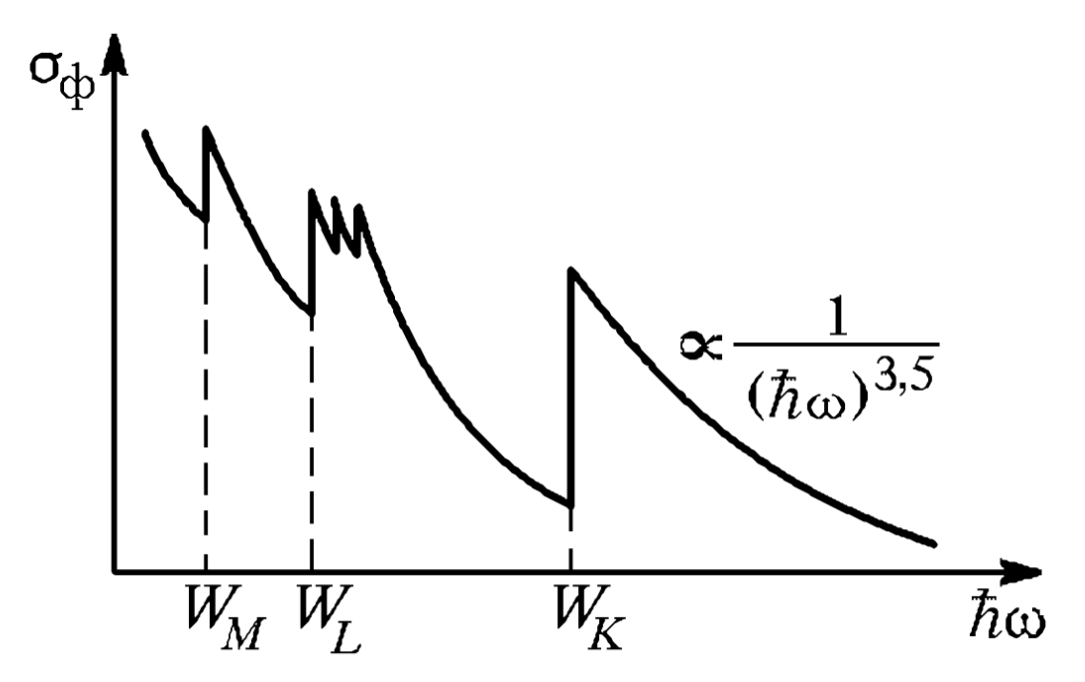
\includegraphics[width=1\linewidth]{01}}
	 \end{wrapfigure}
	\vspace{0.3cm}
	ЗСЭ: $mc^2+\hbar \omega_0=\gamma mc^2+\hbar \omega_1$	
	\vspace{0.3cm}
	
	ЗСИ: $\frac{\hbar\omega_0}{c}=\frac{\hbar\omega_1\cos\theta}{c}+\gamma mvcos\varphi$
	\vspace{0.3cm}
	
	~~~~~~~~~$\gamma mvsin\varphi=\frac{\hbar\omega_1}{c}sin\theta$
	
	\pagebreak
	Переходя от $\omega_0$, $\omega_1$ к $\lambda_0$, $\lambda_1$:
	
	\begin{equation}
	\Delta\lambda=\lambda_1-\lambda_0=\dfrac{h}{mc}(1-\cos\theta)=\Lambda_k(1-\cos\theta)
	\end{equation}
	
	$\Lambda_k=\dfrac{h}{mc}=2,42\cdot 10^{-10}$ см - комптоновская $\lambda$ электрона
	
	
	\vspace{3mm}
		При рассеянии квантов невысокой (1$\div$10 кэВ) энергии часть электронов ведёт себя как связанные, а часть - как свободные, т. е. одновременно наблюдаются релеевское и комптоновское рассеяния.
		
		Цель работы - проверка соотношения (1):
		
		\begin{equation*}
		~~~\frac{1}{\varepsilon(\theta)}-\frac{1}{\varepsilon_0}=1-\cos\theta, ~~~~~~ 
		\varepsilon_0=\frac{E_0}{mc^2}
		\end{equation*}
		
	
	\section{Экспериментальная установка}
	
	
		\begin{figure} [tbh]
			\centering
		{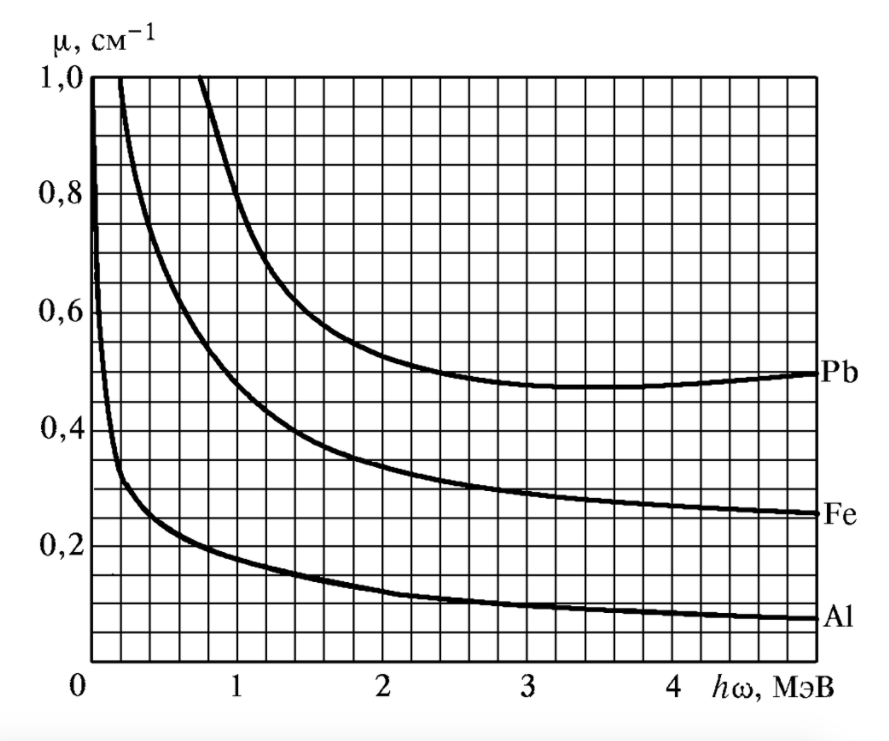
\includegraphics[width=0.6\linewidth]{02}}
			\caption{Блок-схема установки по изучению рассеяния $\gamma$-квантов: 1 - источник излучения ($^{137}$Cs), 2 - графитовая мишень, 3 - фотоэлектронный умножитель (ФЭУ), 4 - сцинтиллятор, 5 - свинцовый коллиматор, 6 - лимб }
		\end{figure}

	\begin{figure}[H]
		\centering
		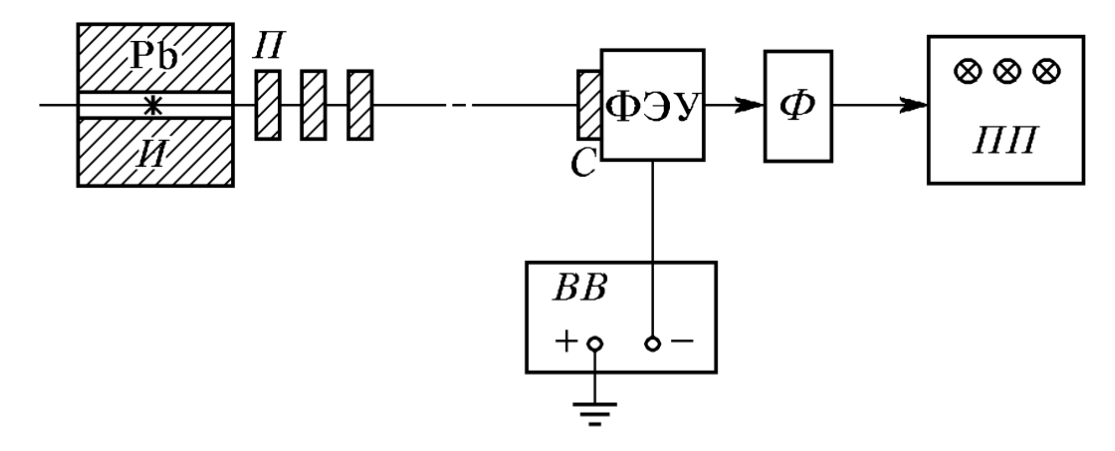
\includegraphics[width=0.4\linewidth]{03}
		\caption{Блок-схема измерительного комплекса: Д- дисплей, ПР - принтер, ВСВ - высоковольтный выпрямитель, УА - усилитель-анализатор, КЛ - клавиатура}
	\end{figure}
			
	%Источник излучения испускает $\gamma$-лучи с энергией 662 кэВ. Кванты, испытавшие %комптоновское рассеяние в мишени, регистрируются сцентилляционным счётчиком.

	\section{Ход работы}
	Устанавливая сцинтилляционный счётчик под разными углами $\theta$ к первоначальному направлению полёта $\gamma$-квантов, сняли амплитудные спектры и определили положение фотопиков для каждого угла.
	
		
			\begin{table}[H]
				\caption{Результаты измерений:}
				\hspace{0.7cm}
				\begin{tabular}{|l||c|c|c|c|c|c|c|c|c|c|c|c|c|}
					\hline
					Угол,$^\circ$ & 0 & 11 & 20 & 30 & 40 & 50 & 60 & 70 & 80 & 90 & 100 & 110 & 120 \\ \hline
					Канал & 986 & 891 & 803 & 734 & 691 & 603 & 526 & 502 & 440 & 414 & 370 & 349 & 316 \\ \hline
					
				\end{tabular}
			\end{table}
			
		\section{Обработка данных}
				\begin{enumerate}
			\item Построили график зависимости $\dfrac{1}{N(\theta)}$ от $(1-\cos\theta)$ и провели через точки наилучшую прямую:
			
			\begin{figure} [H]
				\centering
			{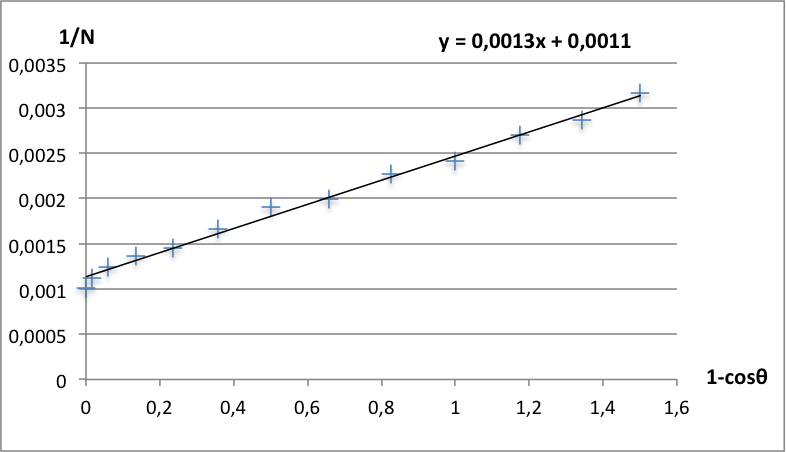
\includegraphics[width=0.7\linewidth]{04}}
				\caption{График зависимости  ~~$\dfrac{1}{N(\theta)}-\dfrac{1}{N(0)}= A(1-\cos\theta)$ }
			\end{figure}
			
			Погрешности аппроксимации, рассчитанные методом наименьших квадратов: ($y=Ax+b$): $\frac{\sigma A}{A} \approx 0,023$; $\frac{\sigma b}{b} \approx 0,014$.
			
			\item С помощью графика определили коэффициент пропорциональности между N($\theta$) и $\varepsilon(\theta)$: A = $\frac{\varepsilon}{N}\approx0,0013$.
			
			
			\item Перейдя от переменной $\varepsilon=\frac{E}{mc^2}$ к энергии E, получаем, что энергия частицы, на которой происходит рассеяние, находится по формуле:
			
			\begin{equation}
			mc^2=E_\gamma\cdot\dfrac{N(90)}{N(0)-N(90)}, 
			\end{equation}
			где $E_\gamma$ - энергия $\gamma$-лучей, рассеянных источником.
			
			При этом значения  $ N(0)$ и $N(90) $ используем полученные из графика (а не полученные непосредственно при измерениях), так как эти значения учитывают измерения, сделанные под другими углами.
			
			$N_\text{наил.}(0)\approx909,09$,
			$N_\text{наил.}(90)\approx416,67$
			
			Полученная энергия:
			\begin{equation*}
			E_{\text{эксп.}}=mc^2=662\text{кэВ}\cdot\frac{416,67}{909,09-416,67}\approx560 ~ \text{кэВ}
			\end{equation*}
			
			\item Рассчитаем погрешности измерений:
			
		\begin{equation*}
		\dfrac{\sigma N(0)}{N(0)}=\dfrac{\sigma b}{b}\approx0,014
		\end{equation*}
			
		\begin{equation*}
	\dfrac{\sigma N(90)}{N(90)}=\sqrt{\left(\frac{\sigma b}{b}\right)^2 + \left(\frac{\sigma A}{A}\right)^2}=\sqrt{(0,014)^2 + (0,023)^2}\approx0,027
		\end{equation*}
		
			
		\begin{equation*}
		\hspace{-1,3cm}\dfrac{\sigma E}{E}=\sqrt{\left(\frac{\sigma N(90)}{N(90)}\right)^2+\left(\frac{\sigma N(0)+\sigma N(90)}{N(0)-N(90)}\right)^2}=\sqrt{(0,027)^2+\left(\frac{11,25+12,73}{909,09-416,67}\right)^2}\approx0,056=5,6\%
		\end{equation*}	
		
		\vspace{5mm}
		С учётом погрешностей:
		\begin{equation*}
		\underline{E_{\text{эксп.}} = 560\pm32 ~\text{кэВ}}
		\end{equation*}
			
		Энергия покоя электрона:
		\begin{equation*}
		\underline{E_{\text{электр.}}=mc^2=9,1\cdot 10^{-31}\cdot (3\cdot 10^8)^2 \approx 511~\text{кэВ}}
		\end{equation*}
		
		\end{enumerate}
		
	\section{Вывод}
	Исследовали энергетический спектр $\gamma$-квантов, рассеянных на графите.  Используя полученные данные, построили график зависимости $\frac{1}{N(\theta)}$ от $(1-\cos\theta)$, где N - номер канала в анализаторе, $\theta$ - угол рассеяния. Полученная зависимость оказалась линейная. С её помощью определили энергию покоя частицы, на которой происходит рассеяние: $E_{\text{эксп.}}=560\pm32~\text{кэВ}$. В пределах погрешностей полученная величина оказалась близкой к энергии покоя электрона: $E_{\text{электр.}}\approx511~\text{кэВ}$, то есть, как и предполагалось, рассеяние происходит на электронах. Погрешность вычисления энергии составила 5,6\%.
	
	
	
\end{document}